\def\firstcircle{(0,0) circle (3cm)}
\def\secondcircle{(2,3.4) circle (3cm)}
\def\thirdcircle{(4,0) circle (3cm)}

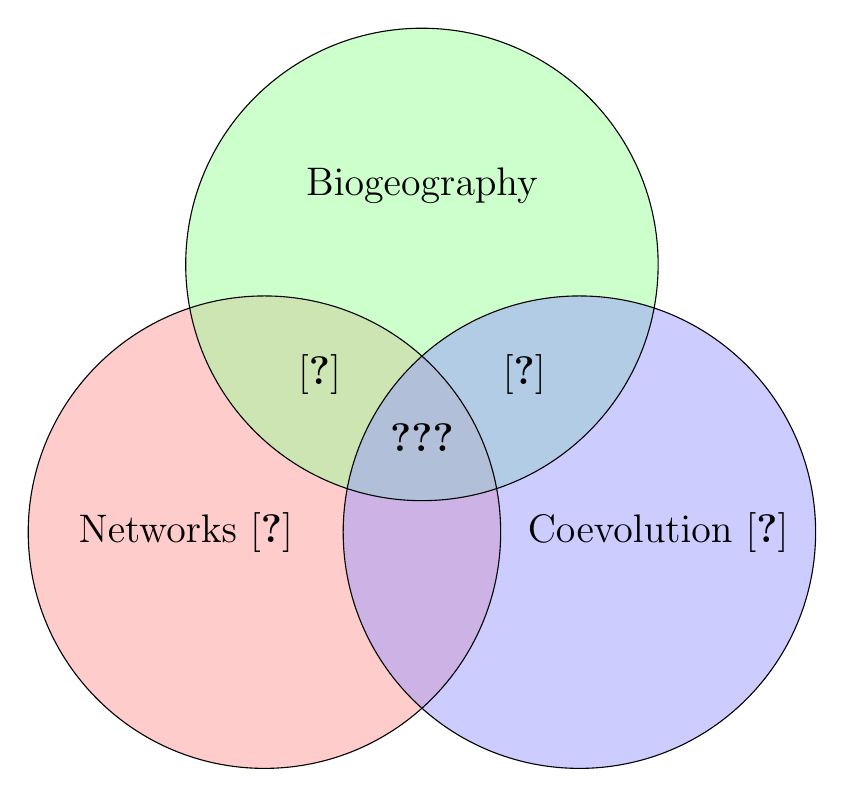
\begin{tikzpicture}
    \begin{scope}[fill opacity=0.5]
        \fill[red!40] \firstcircle;
        \fill[green!40] \secondcircle;
        \fill[blue!40] \thirdcircle;
        \draw \firstcircle node[below] {};
        \draw \secondcircle node [above] {};
        \draw \thirdcircle node [below] {};
    \end{scope}
    %% Draw the labels
    \draw (5,0) node {\Large Coevolution \cite{Thompson1994}};
    \draw (2,4.4) node {\Large Biogeography};
    \draw (-1,0) node {\Large Networks \cite{Pascual2006}};
    
    %% What we don't know
    \draw (2,1.2) node {\bfseries\Large ???};
    
    %% References about what we know
    \draw (3.3,2) node {\Large\protect\cite{Thompson2005}};
    \draw (0.7,2) node {\Large\protect\cite{Gravel2011c}};
    
\end{tikzpicture}